%%%%%%%%%%%%%%%%%%%MAIN_OPTIONS%%%%%%%%%%%%%%%%%%%
\documentclass[a4paper, 14pt]{article}

%% Работа с русским языком
\usepackage{cmap}					% поиск в PDF
\usepackage{hyperref}				% гиперссылки
\usepackage[warn]{mathtext} 		% русские буквы в формулах
\usepackage[T2A]{fontenc}			% кодировка
\usepackage[utf8]{inputenc}			% кодировка исходного текста
\usepackage[english,russian]{babel}	% локализация и переносы

%% Дополнительная работа с математикой
\usepackage{amsfonts,amssymb,amsthm,mathtools} % AMS
\usepackage{amsmath}
\usepackage{icomma} % "Умная" запятая: $0,2$ --- число, $0, 2$ --- перечисление

%% Номера формул
%\mathtoolsset{showonlyrefs=true} % Показывать номера только у тех формул, на которые есть \eqref{} в тексте.

%%FONTS_Packadges
\usepackage{euscript} % Шрифт Евклид
\usepackage{mathrsfs} % Красивый матшрифт

%% Свои команды
\DeclareMathOperator{\sgn}{\mathop{sgn}}

%% Перенос знаков в формулах (по Львовскому)
\newcommand*{\hm}[1]{#1\nobreak\discretionary{}
	{\hbox{$\mathsurround=0pt #1$}}{}}

%%% Работа с картинками
\usepackage{graphicx}  % Для вставки рисунков
\graphicspath{{pictures/}{images2/}}  % папки с картинками
\setlength\fboxsep{3pt} % Отступ рамки \fbox{} от рисунка
\setlength\fboxrule{1pt} % Толщина линий рамки \fbox{}
\usepackage{wrapfig} % Обтекание рисунков и таблиц текстом
\usepackage[section]{placeins}
\usepackage{subcaption}

%% Работа с таблицами
\usepackage{array,tabularx,tabulary,booktabs} % Дополнительная работа с таблицами
\usepackage{longtable}  % Длинные таблицы
\usepackage{multirow} % Слияние строк в таблице

%%Links
\hypersetup{
	colorlinks=true,
	linkcolor=black,
	filecolor=magenta,      
	urlcolor=blue,
}

%%% Программирование
\usepackage{etoolbox} % логические операторы

%%% Страница
\usepackage{extsizes} % Возможность сделать 14-й шрифт
\usepackage{geometry} % Простой способ задавать поля
\geometry{top=25mm}
\geometry{bottom=35mm}
\geometry{left=20mm}
\geometry{right=20mm}
\usepackage{indentfirst}
%
\usepackage{fancyhdr} % Колонтитулы
\pagestyle{fancy}
\renewcommand{\headrulewidth}{0mm}  % Толщина линейки, отчеркивающей верхний колонтитул
%\lfoot{Нижний левый}
%\rfoot{Нижний правый}
%\rhead{Верхний правый}
%\chead{Верхний в центре}
%\lhead{Верхний левый}
% \cfoot{Нижний в центре} % По умолчанию здесь номер страницы

\usepackage{setspace} % Интерлиньяж
%\onehalfspacing % Интерлиньяж 1.5
%\doublespacing % Интерлиньяж 2
%\singlespacing % Интерлиньяж 1

\usepackage{multicol,caption}

\newenvironment{Figure}
{\par\medskip\noindent\minipage{\linewidth}}
{\endminipage\par\medskip}

\usepackage{enumitem}
\usepackage{amssymb}
\usepackage{xcolor}
%%% Зачеркнутый текст
\usepackage[normalem]{ulem}
\usepackage{xurl}



\begin{document}

	\title{		\textbf{\textit{Победит \#398}} 
		
		Cегментация пустот сплава WC-Co}

	\author{$ Д.Г. Каграманян^1, Д.Ю. Камалова^2, Б.Б. Страумал^3, Л.Н. Щур^4$}
	\date{\today}
	\maketitle

	\hfill
	\begin{minipage}{1\textwidth}
			\flushleft
	    $^1$исследователь,dgkagramanyan@edu.hse.ru\\
	    $^2$исследователь,dyukamalova@edu.hse.ru \\
	    $^3$соруководитель,straumal@issp.ac.ru\\
   	 	$^4$руководитель,levshchur@gmail.com\\



	\end{minipage}%

	\section{Аннотация}
	
	Для успешного решения задачи сегментации зерен сплава WC-Co, поставленной в работе \cite{david}, необходимо выделить 
	пустоты микроструктуры (рис. \ref{fig:orig}) и затем составить граф из вершин, находящихся в углах пустот. При помощи полученного графа, который является периметром,  можно посчитать статистическую информацию и выделить зерна сплава.
	
	\begin{figure}[h]
		\center{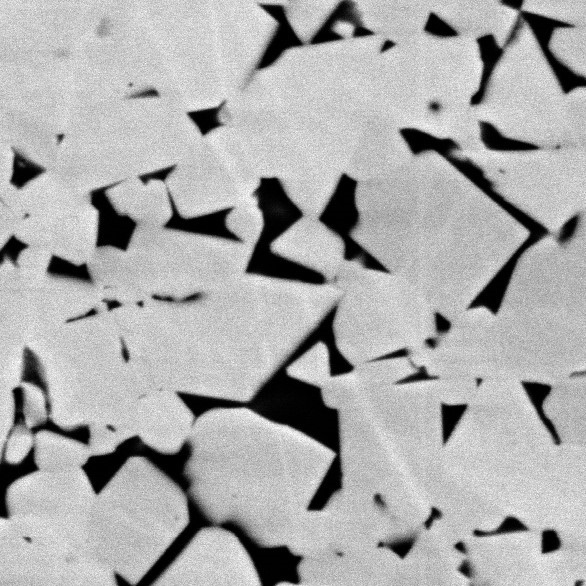
\includegraphics[scale=0.3]{segment_images/original}}
		\caption{Микроструктура сплава WC-Co. Белые участки - зерна, черные - связующее вещество(пустота)  }
		\label{fig:orig}
	\end{figure}
	



	\section{Задача}
	
	Нужно на каждой пустоте разметить вершины углов и соединить их так, чтобы они образовали линию периметра. Иными словами нужно создать полигон на основе координат точек углов.
	
	\section{Предобработка данных}
	\subsection{Первичная обработка изображений}
	
	Самой удачной комбинацией оказались последовательные шаги:
	\begin{itemize}
		
		\item комбинация левой и правой части исходного изображения
		
		\item медианный фильтр
		
		\item бинаризация Отсу
		
		\item карта градиентов
		
	\end{itemize}

	Итоговое изображение вычисляется по формуле \ref{image_eq}.
	
	\begin{equation}
		\label{image_eq}
		\overline{бинаризованное\;изображение}+ карта\;градиентов
	\end{equation}

	Без использования в итоговом изображении градиентов плохо работает детектор углов, а без бинаризованного изображения теряются значения пикселей пустот и не получается выделить отдельную пустоту в индивидуальный регион.
	
	\begin{figure}[h]
		\begin{center}
			\begin{minipage}[h]{0.4\linewidth}
				\center{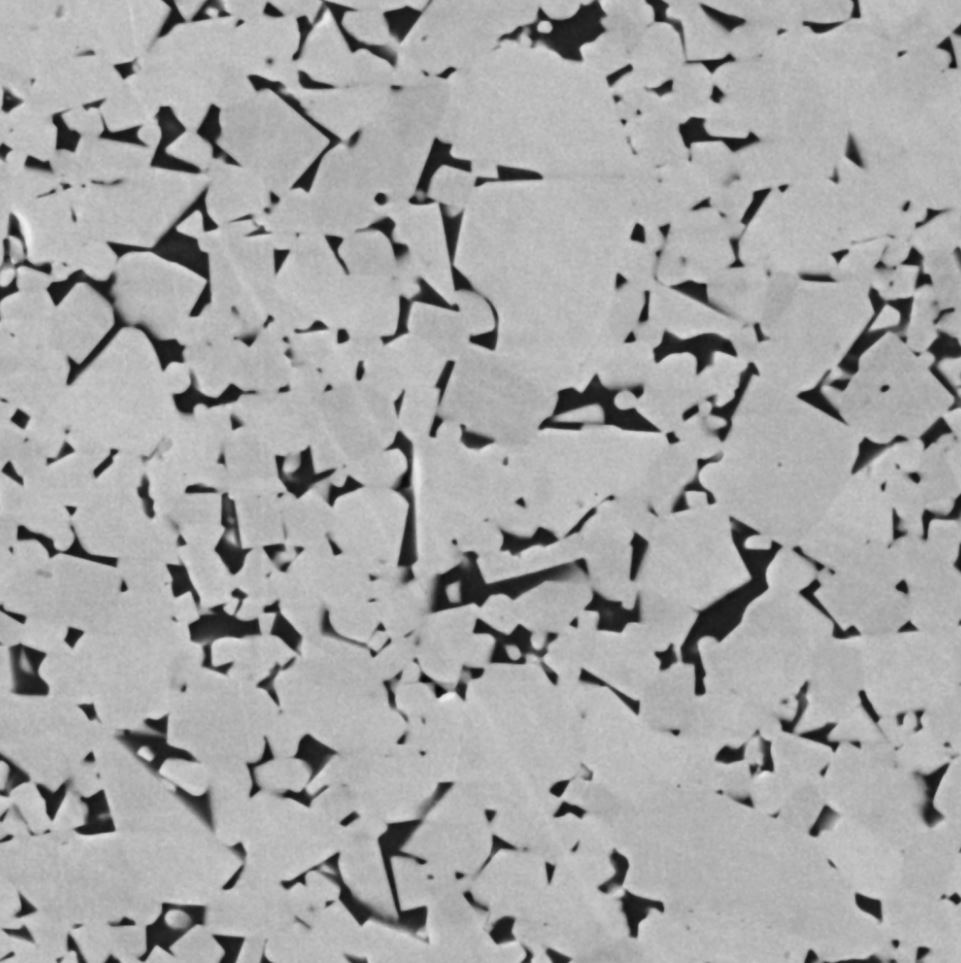
\includegraphics[scale=0.2]{segment_images/denoised2}}
				\caption{Микроструктура после медианного фильтра}
				\label{ris:media}
			\end{minipage}
			\hfill
			\begin{minipage}[h]{0.4\linewidth}
				\center{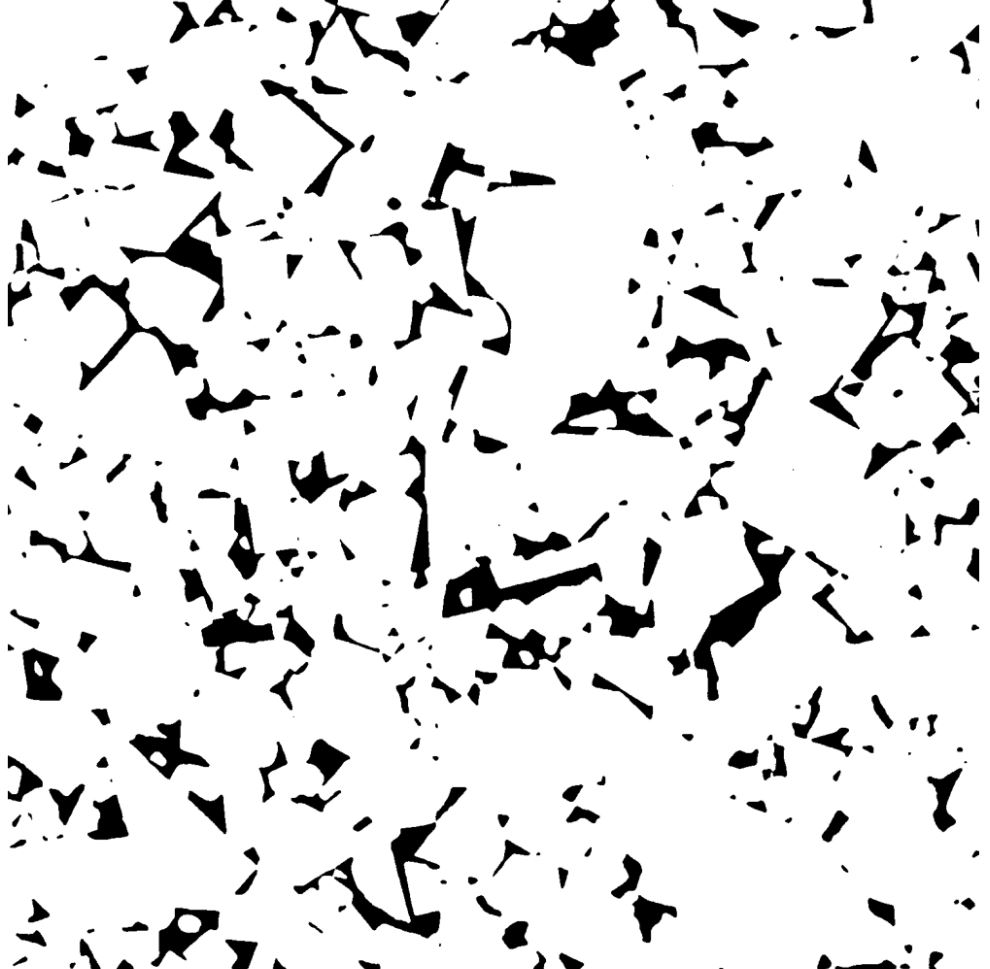
\includegraphics[scale=0.2]{segment_images/binary2}}
				\caption{Бинаризация Отсу}
				\label{fig:otsu}
			\end{minipage}
		\end{center}
	\end{figure}

\begin{figure}[h]
	\begin{center}
		\begin{minipage}[h]{0.4\linewidth}
			\center{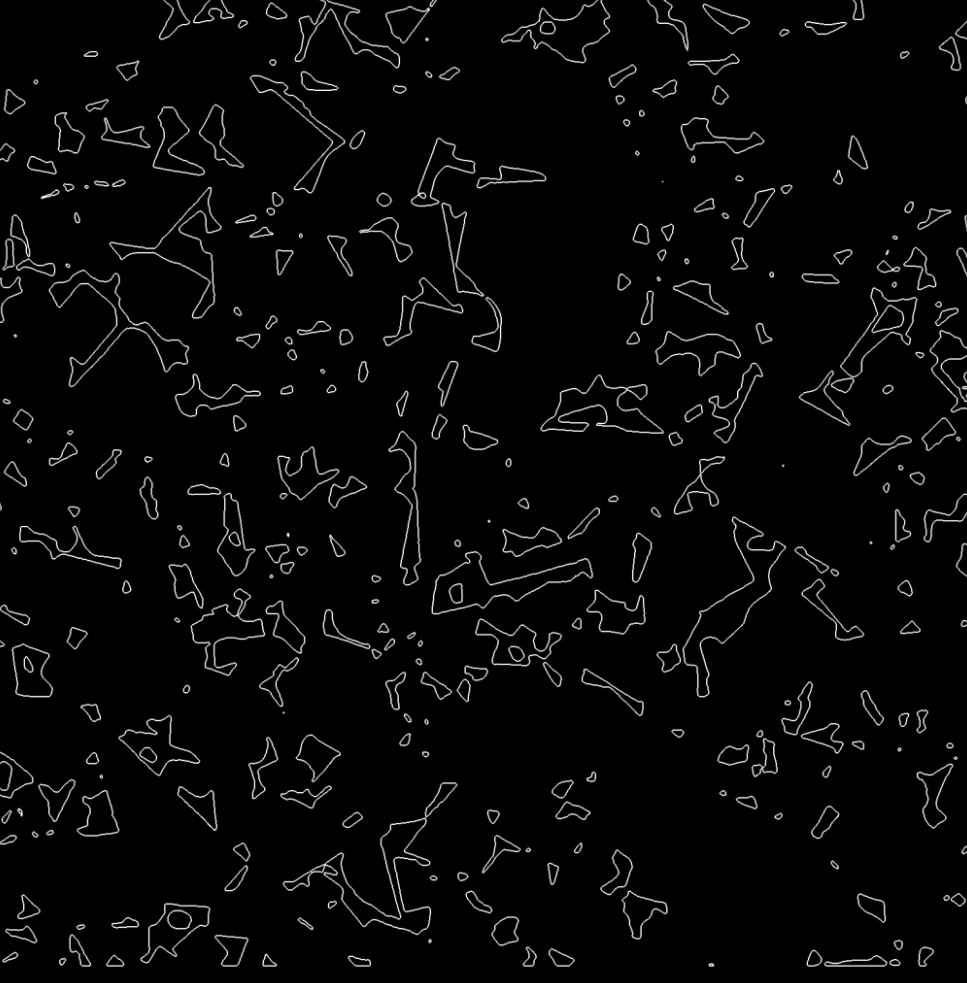
\includegraphics[scale=0.2]{segment_images/grad2}}
			\caption{Карта градиентов}
			\label{ris:grad}
		\end{minipage}
		\hfill
		\begin{minipage}[h]{0.4\linewidth}
			\center{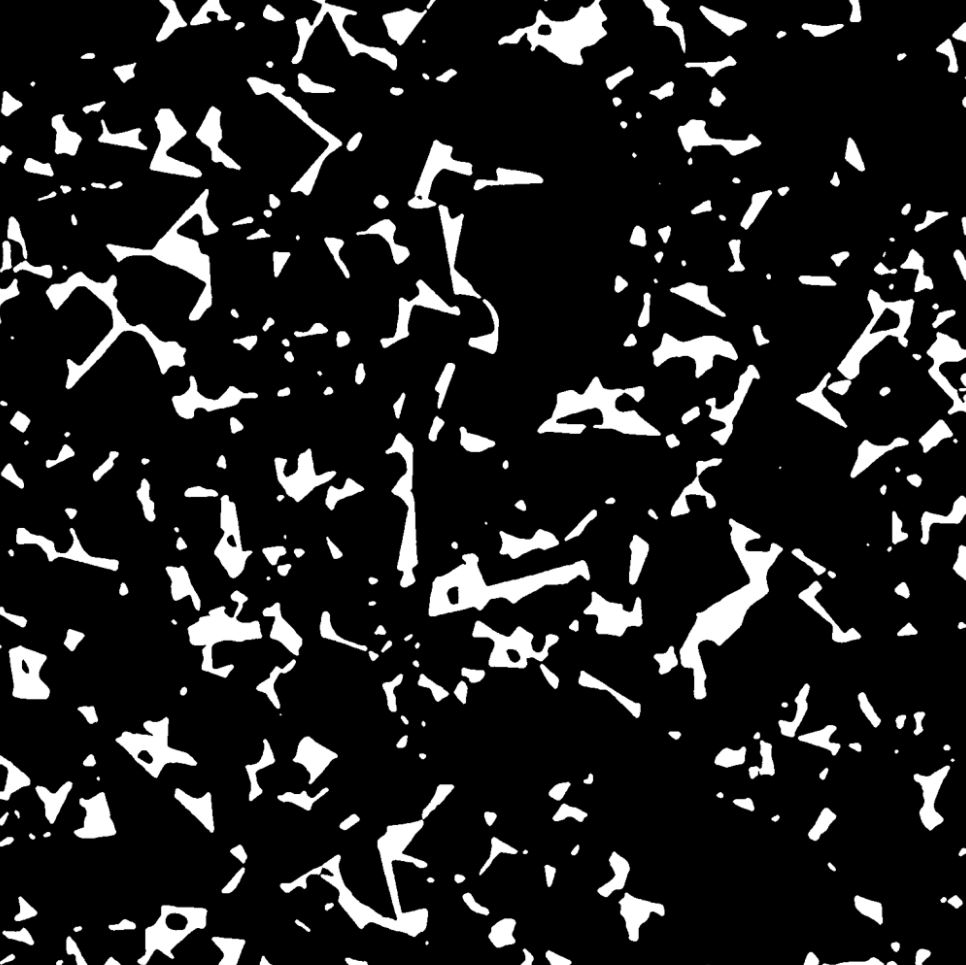
\includegraphics[scale=0.2]{segment_images/image2}}
			\caption{Итоговое изображение}
			\label{fig:result}
		\end{minipage}
	\end{center}
\end{figure}

\subsection{Разметка углов}
\label{corner_mark}
После выделения пустот необходимо разметить вершины углов (рис. \ref{fig:corners}). 
Воспользуеся детектором Ши-Томаси \cite{corners}.

Его принцип работы очень сложен и основан на матрицах свертки, анизитропии и аппроксимации границ при помощи гиперболы \cite{detectors}. Результат работы алгоритма - массив координат неупорядоченных точек углов.  

\subsection{Разметка пустот}
\label{region_mark}

Основной принцип - по изображению проходит матрица свертки \cite{ndi_label}, которая выполняет следующие задачи:
\begin{itemize}
	\item считает количество уникальных особенностей
	
	\item дает кажому пикселю свой класс, к которому он принадлежит
\end{itemize}

Как итог - каждый пиксель изображения имеет привязку к определенному классу пустоты (рис. \ref{fig:classes}).

\subsection{Привязка углов к пустотам}

Следующий этап обработки данных - привязка каждого угла к пустоте, на которой она находится. 
Это значит, что у каждой вершины может быть ровно одна привязка к пустоте, но у одной пустоты может быть много вершин. 


\begin{figure}[h]
	\begin{center}
		\begin{minipage}[h]{0.4\linewidth}
			\center{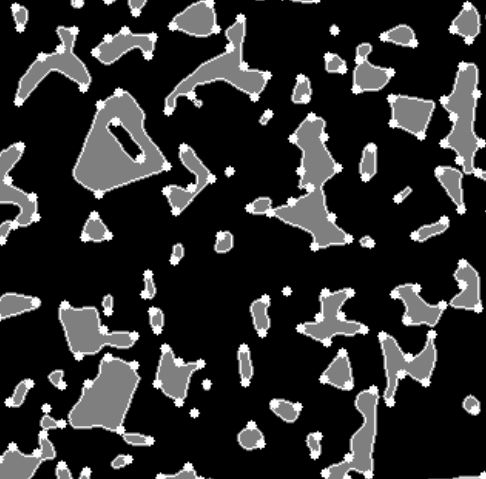
\includegraphics[scale=0.6]{segment_images/corners3}}
			\caption{Размеченные углы пустот (белые точки)}
	\label{fig:corners}
		\end{minipage}
		\hfill
		\begin{minipage}[h]{0.4\linewidth}
			\center{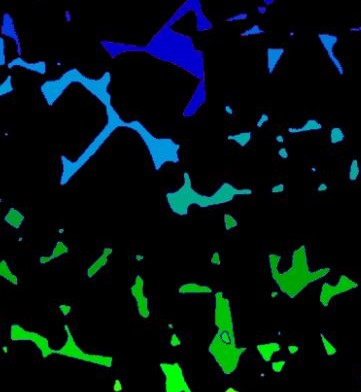
\includegraphics[scale=0.75]{segment_images/classes1}}
			\caption{Разметка пустот. Каждый цвет обозначает индивидуальный класс}
			\label{fig:classes}
		\end{minipage}
	\end{center}
\end{figure}

\section {Создание линий периметра}
\subsection{Обход всех вершин}
Зададим метрики для ребер:
\begin{itemize}
	\item mean(point1,point2,R) - среднее значение пикселей в прямоугольнике длины $\| point1-point2\|$ и ширины 2*R
		\label{mean}
	
	\item dist(point1,point2)- расстояние $\| point1-point2\|$ между двумя вершинами, образующими ребро
\end{itemize}

Основной принцип итеративного обхода - фиксирование одной вершины и обход всех остальных относительно первой. 
При успешном определении следующей точки, она фиксируется, а первая удаляется из списка доступных. Итерация продолжается до конца списка доступных вершин. Количество итераций можно строго описать  в виде суммы переборов для каждой вершины региона (ур. \ref{sum}). Сложность алгоритма $О(N^2)$ .

\begin{equation}
	\label{sum}
	(N-1)+(N-2)+..=\sum\limits_{i=1}^{N-1} (N-i)={1\over{2}}(N-1)N
\end{equation}
где N - количество вершин(углов) в пустоте сплава.

Для вычисления метрики среднего значения \ref{mean} обозначим вектор ребра двух вершин $\overline{L}=(L_x;L_y)=(x_2-x_1;y_2-y_1)$.
Получим координаты второй стороны (ширины) прямоугольника. Для этого пустим из точки $(x1;y1)$ вектор $\overline{А}=(А_x;А_y)=(a_x-x_1;a_y-y_1)$.

Решим систему уравнений (ур. \ref{system}) и получим (ур. \ref{def} ) координаты  $a_x\; и\; a_y$ второй точки вектора $\overline{A}$.


\begin{equation}
	\label{system}
	\begin{cases}
		(a_x-x_1)^2+(a_y-y_1)^2=R^2 
		\\
		(a_x-x_1)L_x+(a_y-y_1)L_y=0
	\end{cases}
\end{equation}
\begin{equation}
	\label{def}
		a_x=x_1-{{RL_y}\over{\sqrt{{L_x}^2+{L_y}^2}}}\;
		a_y=y_1+{{RL_x}\over{\sqrt{{L_x}^2+{L_y}^2}}}
\end{equation}

\begin{figure}[h]
	\center{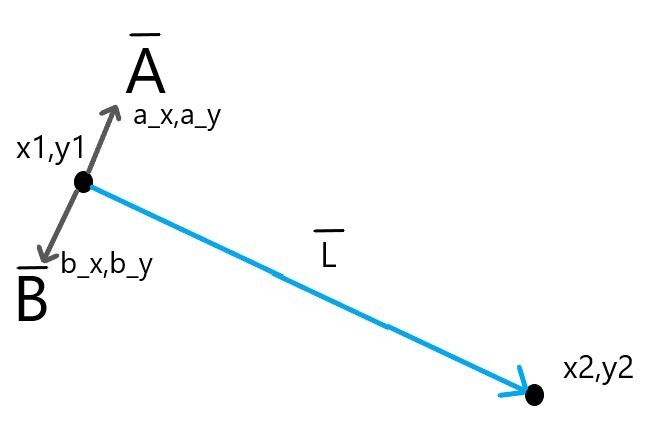
\includegraphics[scale=0.47]{segment_images/lines}}
	\caption{Вектора , использвоанные при построении прямоугольника между точками}
	\label{fig:lines}
\end{figure}

Для вектора $\overline{B}$ действия идентичны, как для вектора $\overline{A}$. 

Получим координаты прямой между точками $(a_x;a_y)\;и \;(b_x;b_y)$ при помощи алгоритма Брезенхема \cite{line}.
Пройдемся по каждой точке полученной прямой: построим  из $(x^i;y^i)$ в $(x^i+L_x;y^i+L_y)$ новую прямую, которая будет
являться i-тым слоем прямоугольника. Завершив проход по всем точкам, получим правильный и удобный для итерации массив точек прямоугольника. Алгоритм учитывает наклон фигуры.     


\subsubsection{Простое комбинирование метрик}
\label{sec:combine} 
Принцип работы - сложение или умножение двух метрик с весовыми коэффициентами.
 Расстояние между вершинами нормируется относительно максимальной или средней длины ребра в пустоте. 
Алгоритм итеративно ищет ту вершину, для которой суммарная метрика наименьшая. 

Результат - успешная сегментация только на вершинах,находящихся на выпуклой части полигона (рис. \ref{fig:good}). 
При наличии тонкой шейки или отклонения формы пустоты от эллипса происходит самопересечение (рис. \ref{fig:bad}). Изменение весовых коэффициентов дает прирост эффективности
сегментации для одних регионов, но ухудшает для других. 

\begin{figure}[h]
	\begin{center}
		\begin{minipage}[h]{0.4\linewidth}
			\center{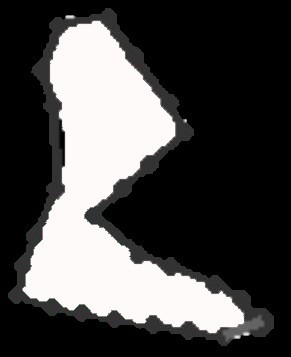
\includegraphics[scale=0.65]{segment_images/good_segmented}}
			\caption{Верное соединение вершин региона}
			\label{fig:good}
		\end{minipage}
		\hfill
		\begin{minipage}[h]{0.4\linewidth}
			\center{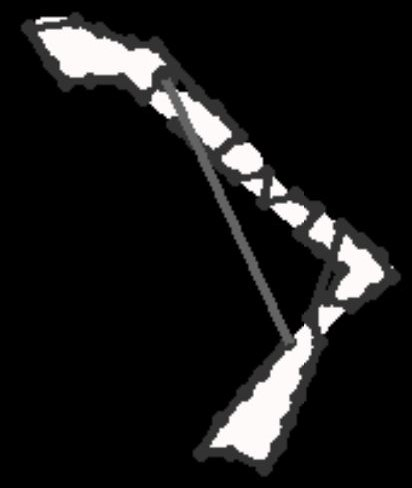
\includegraphics[scale=0.5]{segment_images/bad_segmented}}
			\caption{Неверное соединение вершин региона}
			\label{fig:bad}
		\end{minipage}
	\end{center}
\end{figure}

\subsubsection{F-мера} 
Принцип работы - f мера (ур. \ref{eq:f-mera}) комбинация двух метрик А и В с различным значением коэффициента $\beta$, который задает вес одной метрики относительно другой.   Расстояние между вершинами нормируется относительно максимальной или средней длины ребра в пустоте. 
Алгоритм итеративно ищет ту вершину, для которой f-мера наибольшая. 
\begin{equation}
	F_\beta={{(1+\beta^2)AB} \over {\beta^2 A+B}}
	\label{eq:f-mera}
\end{equation}



Результат - самопересечение,сегментации нет. При нормировке расстояние заведомо находится нулевом диапазоне значений  из-за большого нормирующего значения. Подбор параметра $\beta$ , как  для весов в разделе \ref{sec:combine}, усложняется неопропорциональным влиянием на процесс сегментации. 

\subsubsection{Последовательное применение метрик} 
\label{future}
Принцип работы - сортировка(по возрастанию) вершин по расстоянию. Затем поиск до первого совпадения вершины с наиболее близким к 0.5 метрики mean (\ref{mean}).
 
Результат - самопересечение,сегментации нет. Разметка углов на изображении может происходить с небольшим сдвигом в область региона. Появляется сдвиг среднего значения пикселей между вершинами. Нет единого $\varepsilon$  для сравнения mean (\ref{mean}) c 0.5, на основе которого можно выявить вершину на границе. Для каждой вершины  $\varepsilon$ лежит в диапазоне от 0.1 до 0.3.

\textbf{Будущее развите}. При использовании динамического определения отклонения среднего значения писелей от 0.5 может быть достигнут хороший результат.


\subsection{Аналитический подход}
Не реализован. 

Интересный, но сложный путь решения \cite{polygon_anal}. Создание полигона только на основе координат нетривиальная задача так как существует множество вариаций линии периметра, проходящей полинии. 
В поставленной задаче помимо координат есть само изображение, которое однозначно определяет форму пустоты. 

\subsection{Геометрическая аппроксимация} 
\subsubsection{Convex hull}
\label{convex}


Простой и рабочий метод для создания грубого полигона \cite{convex_hull}. Принцип работы схож 
с стягиванием вокруг вбитых гвоздей связанной нитки (рис. \ref{fig:convex_hull}).


\begin{figure}[h]
	\center{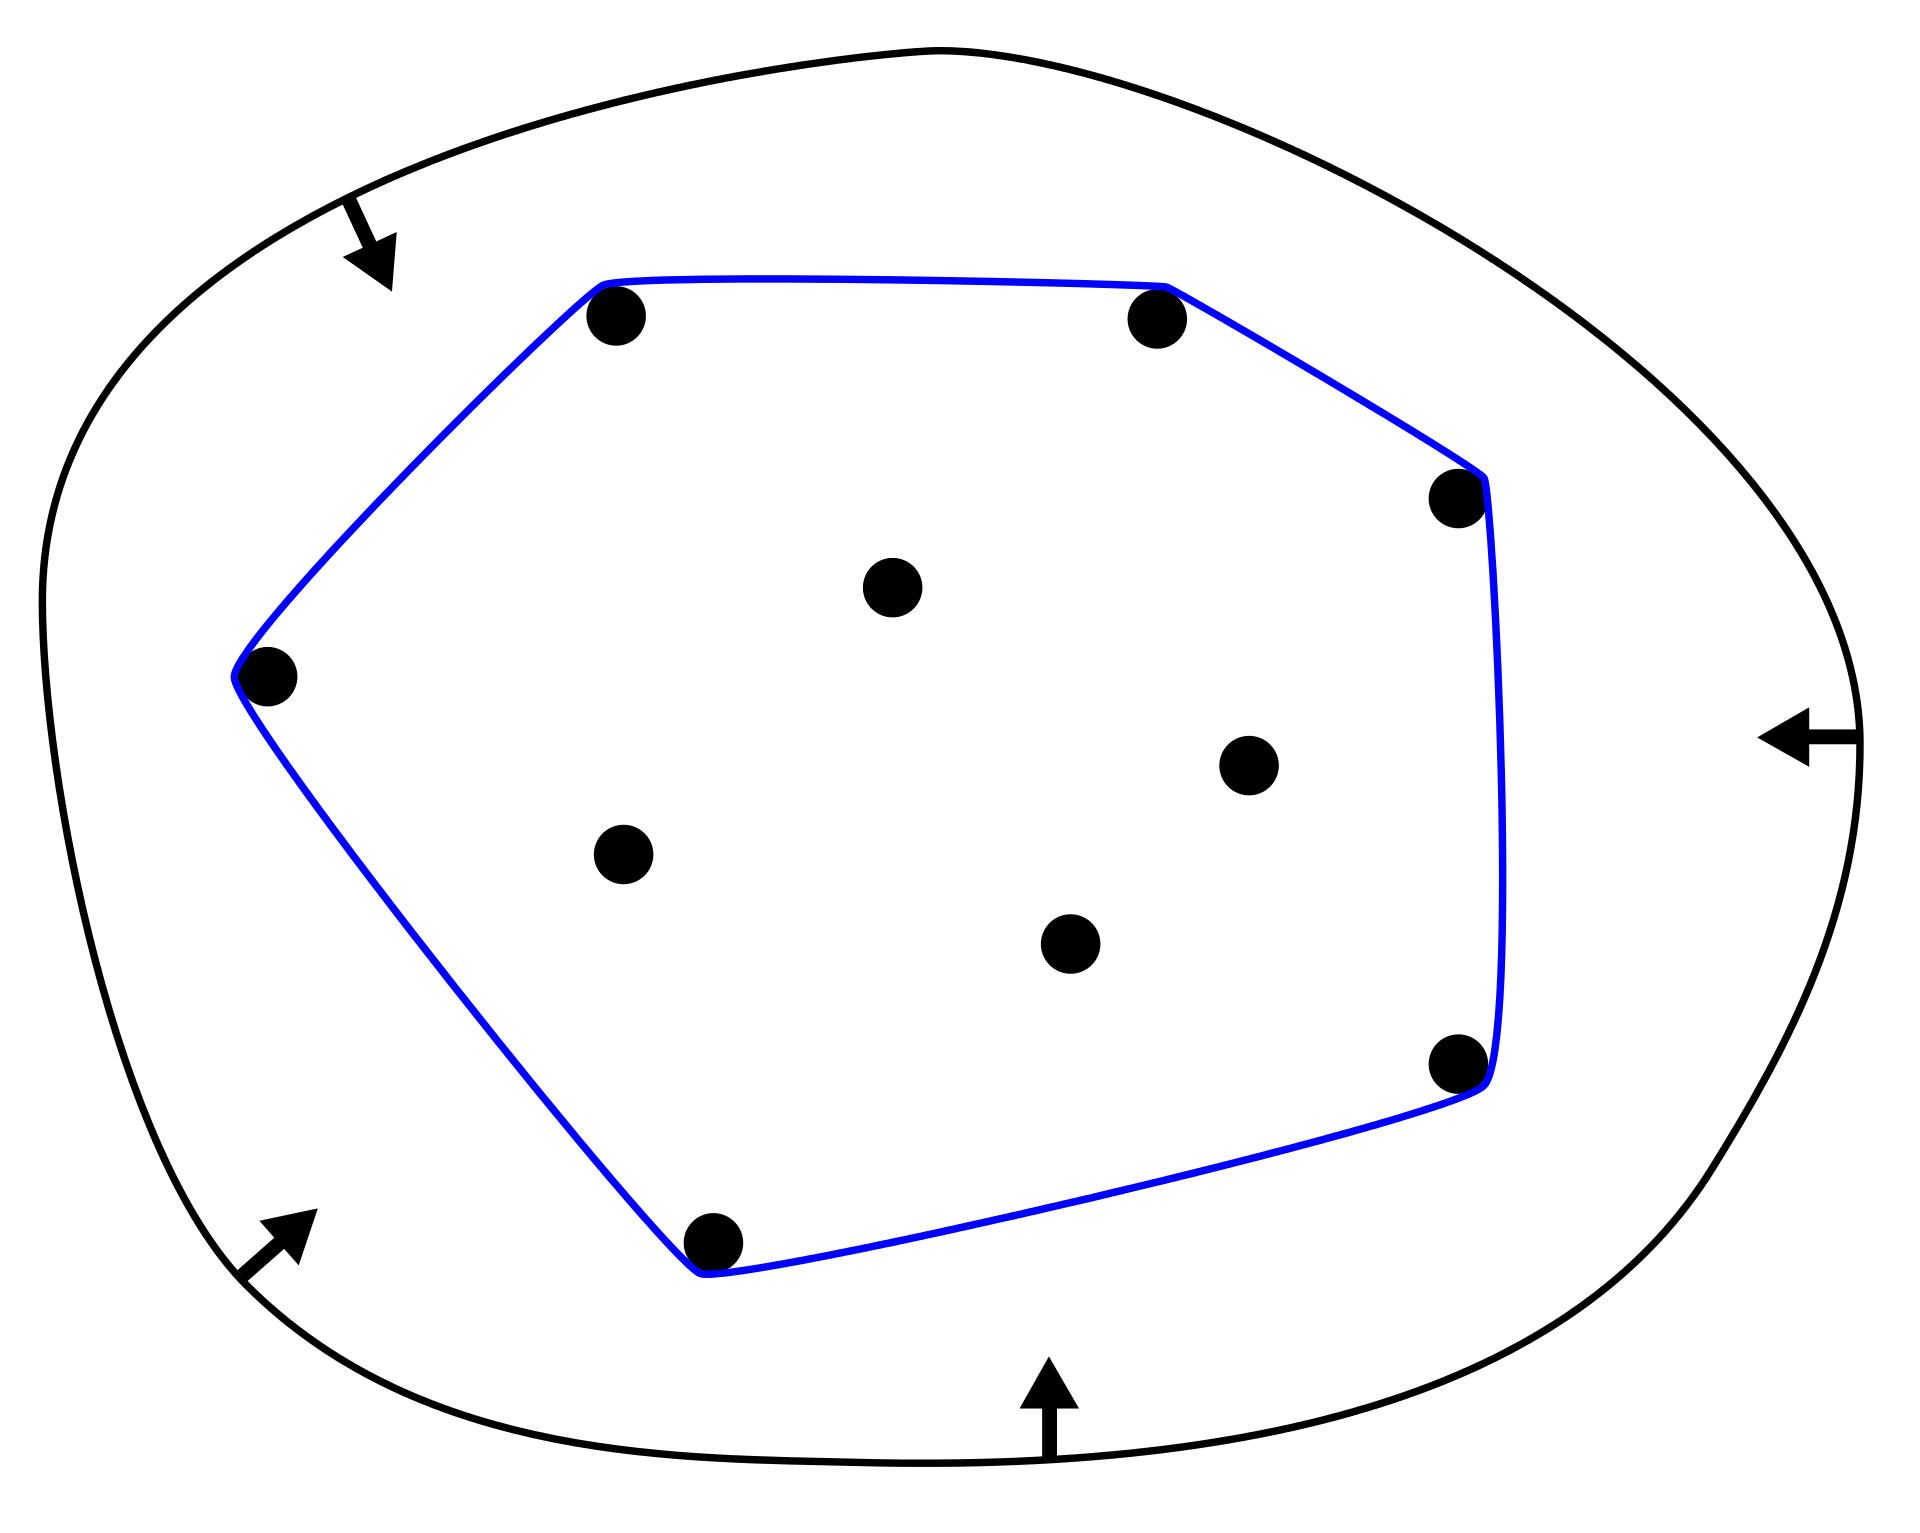
\includegraphics[scale=0.1]{segment_images/convex_hull}}
	\caption{Черные  точки - "вбитые гвозди"\ , черная линия - связанная нитка, которая при стягивании занимает место синей линии}
	\label{fig:convex_hull}
\end{figure}

Результат работы алгоритма - неточное выделение контура пустот. Подходит только для выпуклых регионов(рис. \ref{fig:convex_hull_done}).  
\begin{figure}[h]
	\center{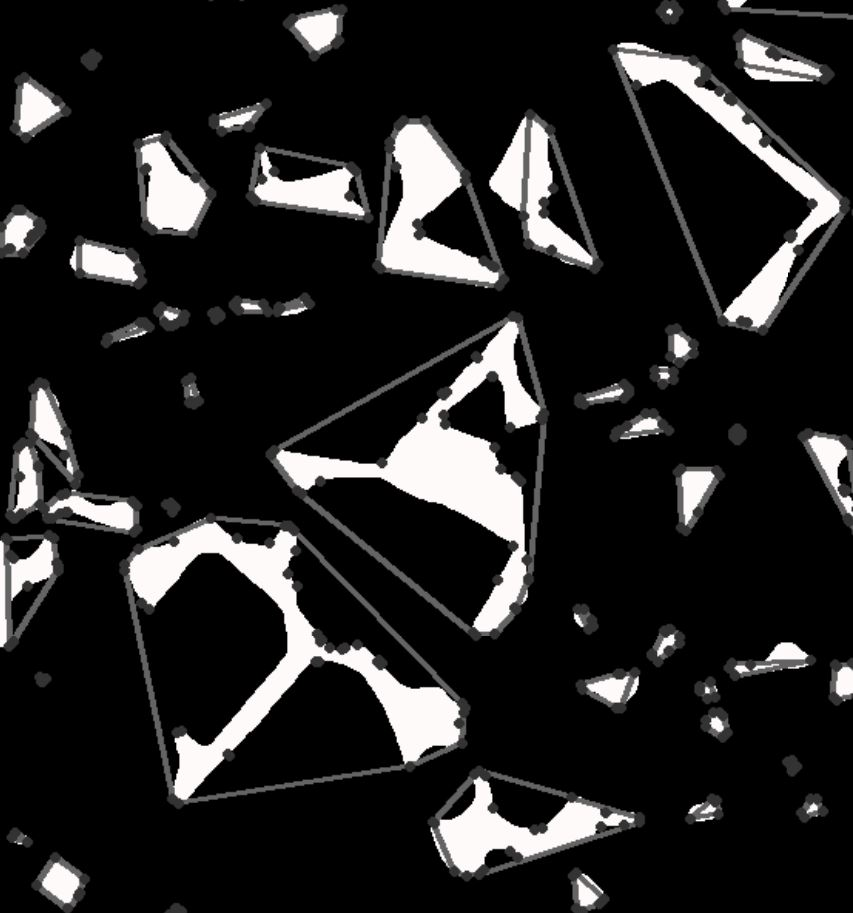
\includegraphics[scale=0.4]{segment_images/convex_hul_done}}
	\caption{Серые линии - периметр пустот, полученный в результате работы convex hull}
	\label{fig:convex_hull_done}
\end{figure}

\subsubsection{Поиск контуров и линейная аппроксимация}
\label{final}
Иной вариант решения задачи.Получим упорядоченный набор пикселей контуров пустот, а затем аппроксимируем их линейной функцией. 

Реализуем последовательность нескольких алгоритмов:
\begin{itemize}
	\item поиск границ детектором Кенни \cite{canny}
	
	\item получение упорядоченного набора пикселей контуров \cite{find_contour}
	
	\item линейная аппроксимация контура \cite{polygon_appx}
\end{itemize}
Сначала детектор границ Кенни выделяет границы у пустот (рис. \ref{fig:canny}). Затем полученные контуры обрабатываются на алгоритмом \cite{find_contour} и потом каждому пикселю контура присваивается порядковый номер. Последний этап - уменьшение количества точек и аппроксимация пикселей с помощью линейной функции (рис. \ref{fig:find_contour}).

Результат - достаточно точное выделение границ пустот при помощи прямых линий и отсутсвие необходимости в предварительной разметке углов.

\begin{figure}[h]
	\begin{center}
		\begin{minipage}[h]{0.4\linewidth}
			\center{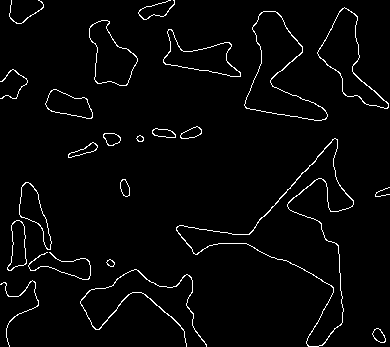
\includegraphics[scale=0.8]{segment_images/edges_resized}}
			\caption{Выделенные методом Кенни контуров пустот}
			\label{fig:canny}
		\end{minipage}
		\hfill
		\begin{minipage}[h]{0.5\linewidth}
			\center{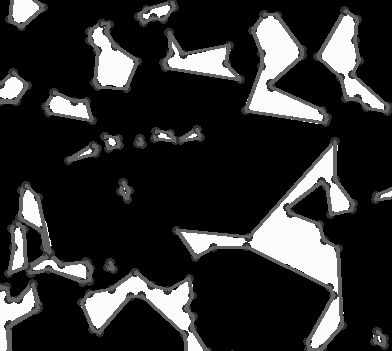
\includegraphics[scale=0.8]{segment_images/lines_resized}}
			\caption{Пустоты с линейно аппроксимированными границами}
			\label{fig:find_contour}
		\end{minipage}
	\end{center}
\end{figure}






\section{Выводы}

Поставленная задача на деле оказалась нетривиальной. Множество популярных методов не смогли показать достаточный уровень точности определения границы. 

Метод из главы \ref{final} показал отличное решение поставленной задачи. При помощи комбинации нескольких алгоритмов удалось выделить границы пустот и получить упорядоченный и линейно приближенный набор пикелей контура.  

\newpage
%далее сам список используевой литературы
\begin{thebibliography}{}
	
	
	\bibitem{ndi_label}   \href{https://docs.scipy.org/doc/scipy/reference/generated/scipy.ndimage.label.html}{scipy.ndimage.label}
	
	\bibitem{polygon_anal}  Hongyun Zhang ,Quanhua Zhao  ,Yu Li   -  \href{https://journals.plos.org/plosone/article?id=10.1371/journal.pone.0230342}{Generation of simple polygons from ordered points using an iterative insertion algorithm}
	
	\bibitem{convex_hull}    \href{https://en.wikipedia.org/wiki/Convex_hull}{Convex hull}

	\bibitem{corners}  Shi-Tomasi   -  \href{https://en.wikipedia.org/wiki/Corner_detection}{Corner detection}
	
	\bibitem{polygon_appx} Ramer,Douglas,Peucker  - \href{https://habr.com/ru/post/448618/}{Ramer–Douglas–Peucker algorithm}
	
	\bibitem{skimage_approx}  \href{https://scikit-image.org/docs/dev/auto_examples/edges/plot_polygon.html#sphx-glr-download-auto-examples-edges-plot-polygon-py} {Approximate and subdivide polygons}
	
	\bibitem{detectors} lightsource
	 -  \href{	https://habr.com/ru/post/244541/} {Детекторы углов}
	

	
	\bibitem{david} Д.Г.Каграманян -  Сегментация зерен сплава WC-Co готовыми инструментами
	
	\bibitem{line}   Брезенхэм   -  \href{https://en.wikipedia.org/wiki/Bresenham%27s_line_algorithm}{Отрисовка линий в двумерного растра}
		
	\bibitem{canny}    John F. Canny    -  \href{https://en.wikipedia.org/wiki/Canny_edge_detector}{Canny edge detector}
		
	\bibitem{canny_habr}   impersonalis   -  \href{https://habr.com/ru/post/114589/}{Выделение границ Канни}
	
	\bibitem{find_contour}  Satoshi Suzuki,Keiichi Abe   -  \href{https://www.sciencedirect.com/science/article/abs/pii/0734189X85900167}{Topological Structural Analysis of Digitized Binary Images by Border Following}
	

		


\end{thebibliography}
	



	
\end{document}